% SC4024 --- Chapter 7: Perceptual, Cognitive & Evaluation (0->100 ground-up)
\chapter{Perceptual, Cognitive \& Evaluation}
\label{ch:perception-evaluation}
\sloppy

\begin{quote}
\emph{``A visualisation is a hypothesis that a picture helps.''} --- Hypotheses need tests. This chapter asks how to know whether a picture actually helps and how the mind works with it.
\end{quote}

\noindent\fbox{\parbox{\dimexpr\linewidth-2\fboxsep-2\fboxrule}{%
\textbf{From zero: we build here, no prior perception or statistics needed.} We start from what eyes do in milliseconds and what memory holds in seconds, then build controlled studies, measures, and analyses, with examples. No prior evaluation experience is required.}}
\vspace{0.4em}

\section*{Learning Outcomes}
After this chapter you will be able to:
\begin{enumerate}[label=(L\arabic*)]
    \item explain pre-attentive pop-out, change blindness, and attention limits;
    \item describe mental models, chunking, cognitive load, and dual-process reasoning;
    \item design a controlled study: hypothesis, variables, tasks, and protocol;
    \item choose measures (accuracy, time, preference, insight) and avoid pitfalls;
    \item analyse results with confidence intervals, t-tests/ANOVA, and effect sizes.
\end{enumerate}

% ============================================================
\section{Beyond the Retina: Attention and Memory}
\label{sec:beyond-retina}
\paragraph{Intuition.} You can spot a red dot instantly, but try finding a red vertical line among red horizontal and blue vertical lines---now you must search deliberately, and if the display flickers you may miss a large change entirely. Seeing is not just optics; it is attention and memory.

\paragraph{Formal view.} \emph{Pre-attentive} features (hue, size, orientation, motion) are processed in parallel ($<$200\,ms, pop-out). \emph{Conjunctions} require serial focal attention. \emph{Change blindness}: large changes go unseen without focused attention, especially during saccades or flicker. \emph{Attention} is a limited spotlight; \emph{working memory} holds $\sim$4 chunks; \emph{long-term memory} stores schemas that chunk complex patterns into one unit.

\begin{definition}[Cognitive concepts]\label{def:cognitive}
\emph{Mental model}: internal representation of data structure built from the picture. \emph{Chunking}: grouping pieces into a unit (e.g.\ a cluster of dots becomes ``the high group''). \emph{Cognitive load}: effort to hold and manipulate chunks; extraneous load from poor design harms insight. \emph{Dual-process}: System~1 (fast, pattern-matched) vs System~2 (slow, analytical); visualisation aims to make correct insights System~1-fast.
\end{definition}

\begin{figure}[h]\centering
\begin{tikzpicture}[scale=0.78,every node/.style={font=\scriptsize}]
% pop-out vs conjunction redux but with RT
\begin{scope}
\node[font=\footnotesize\bfseries] at (1.6,3.6) {Feature search (pop-out)};
\foreach \x in {0.3,0.9,1.5,2.1} \foreach \y in {1.8,2.3,2.8} \fill[blue!55] (\x,\y) circle (0.09);
\fill[red!70] (1.2,2.05) circle (0.11);
\draw[->,thick,green!60!black,>=Stealth] (1.2,1.6) -- (1.2,1.0) node[midway,right,font=\tiny] {$\sim$200\,ms flat};
\node[font=\tiny,fill=green!10,rounded corners=2pt] at (1.6,0.7) {parallel, RT independent of N};
\end{scope}
\begin{scope}[xshift=4.2cm]
\node[font=\footnotesize\bfseries] at (1.6,3.6) {Conjunction search};
\foreach \x in {0.3,0.9,1.5,2.1} \foreach \y in {1.8,2.3,2.8} {
  \pgfmathparse{int(mod(\x*10+\y*10,2))}\let\p\pgfmathresult
  \ifnum\p=0 \fill[blue!55] (\x,\y) circle (0.09);
  \else \fill[blue!55] (\x,\y) rectangle +(0.16,0.16); \fi
}
\fill[red!70] (0.9,2.05) circle (0.09);
\fill[red!70] (1.5,2.3) rectangle +(0.16,0.16);
\draw[->,thick,red!60!black,>=Stealth] (1.2,1.6) -- (1.2,1.0) node[midway,right,font=\tiny] {RT $\propto$ N};
\node[font=\tiny,fill=red!10,rounded corners=2pt] at (1.6,0.7) {serial, slow search};
\end{scope}
% change blindness
\begin{scope}[xshift=8.4cm]
\node[font=\footnotesize\bfseries] at (1.8,3.6) {Change blindness};
\fill[gray!10,draw=gray!40] (0,1.8) rectangle (1.7,3.0);
\foreach \x/\y in {0.4/2.5,0.9/2.2,1.3/2.6} \fill[blue!55] (\x,\y) circle (0.08);
\node[font=\tiny] at (0.85,1.55) {flicker: change missed};
\fill[gray!10,draw=gray!40] (1.9,1.8) rectangle (3.6,3.0);
\foreach \x/\y in {0.4/2.5,0.9/2.2,1.3/2.6} \fill[blue!55] (1.9+\x,\y) circle (0.08);
\fill[red!60] (3.0,2.5) circle (0.08) node[right,font=\tiny] {new};
\draw[<->,thick,>=Stealth,orange!70!black] (1.7,2.4) -- (1.9,2.4) node[midway,above,font=\tiny] {gap};
\node[font=\tiny,fill=orange!10,rounded corners=2pt] at (1.8,0.7) {large changes need attention};
\end{scope}
% working memory
\begin{scope}[xshift=12.2cm]
\node[font=\footnotesize\bfseries] at (1.2,3.6) {Working memory};
\draw[fill=violet!12,draw=violet!40,rounded corners=4pt] (0,1.6) rectangle (2.4,3.0);
\foreach \i in {0,...,3} \fill[blue!18,draw=blue!40] (0.25+0.55*\i,2.0) rectangle +(0.40,0.5);
\node[font=\tiny] at (1.2,1.35) {$\sim$4 chunks};
\node[font=\tiny,fill=violet!8,rounded corners=2pt] at (1.2,0.7) {chunk = cluster, trend};
\end{scope}
\node[font=\tiny,draw=gray!40,fill=yellow!8,rounded corners=2pt,inner sep=3pt] at (6.8,0.2) {\textcolor{green!50!black}{$\blacksquare$ pop-out} \quad \textcolor{red!60!black}{$\blacksquare$ serial} \quad \textcolor{orange!70!black}{$\blacksquare$ blindness} \quad \textcolor{violet!60!black}{$\blacksquare$ memory}};
\end{tikzpicture}
\caption{Perception and attention: feature search is parallel (left); conjunction search is serial (centre-left); change blindness hides large changes without attention (centre-right); working memory holds $\sim$4 chunks (right).}
\label{fig:perception-cog}
\end{figure}

Good design respects these limits: encode the answer in a pre-attentive feature when possible, keep the number of colours and groups small, and avoid flicker or gratuitous animation that induces blindness.

% ============================================================
\section{Designing an Evaluation}
\label{sec:evaluation-design}
\paragraph{Intuition.} Claiming ``my chart is better'' without a test is like claiming a drug works without a trial. A controlled study makes the claim falsifiable: fix a task, vary only the picture, measure what matters.

\begin{definition}[Study anatomy]\label{def:study}
\emph{Research question} $\to$ \emph{hypothesis} (e.g.\ ``position beats angle for ratio judgment''). \emph{Independent variable} (IV): what you vary (encoding). \emph{Dependent variable} (DV): what you measure (accuracy, time, preference, insight). \emph{Controls}: keep data, task, and participants balanced. \emph{Protocol}: within-subjects (each participant sees all conditions, counterbalanced) vs between-subjects; randomised order; training and practice trials; ethics consent.
\end{definition}

Classic tasks: Cleveland--McGill ratio judgment (``what percent is the smaller of the larger?''), Heer--Bostock replication with crowdsourcing, insight diaries for open-ended exploration. Choose tasks that span the taxonomy: value retrieval, comparison, trend, outlier, distribution.

\begin{figure}[h]\centering
\begin{tikzpicture}[scale=0.80,every node/.style={font=\scriptsize}]
\node[draw,thick,fill=teal!14,rounded corners=4pt,minimum width=3.2cm,minimum height=0.9cm,align=center] (q) at (0,3.0) {Research question\\{\tiny ``Does X beat Y?''}};
\node[draw,thick,fill=blue!14,rounded corners=4pt,minimum width=3.2cm,minimum height=0.9cm,align=center] (hyp) at (4.2,3.0) {Hypothesis\\{\tiny $H_0$: no diff; $H_1$: X better}};
\node[draw,thick,fill=orange!14,rounded corners=4pt,minimum width=3.2cm,minimum height=0.9cm,align=center] (iv) at (8.4,3.0) {IV / DV / controls\\{\tiny encoding / accuracy, time}};
\draw[->,thick,>=Stealth] (q)--(hyp); \draw[->,thick,>=Stealth] (hyp)--(iv);
\node[draw,thick,fill=green!14,rounded corners=4pt,minimum width=3.2cm,minimum height=0.9cm,align=center] (proto) at (0,1.4) {Protocol\\{\tiny within/between, counterbalance}};
\node[draw,thick,fill=violet!12,rounded corners=4pt,minimum width=3.2cm,minimum height=0.9cm,align=center] (run) at (4.2,1.4) {Run study\\{\tiny consent, training, trials}};
\node[draw,thick,fill=yellow!16,rounded corners=4pt,minimum width=3.2cm,minimum height=0.9cm,align=center] (anal) at (8.4,1.4) {Analyse\\{\tiny CI, t-test/ANOVA, effect}};
\draw[->,thick,>=Stealth] (iv) -- (proto) node[midway,above,font=\tiny,sloped] {operationalise};
\draw[->,thick,>=Stealth] (proto)--(run); \draw[->,thick,>=Stealth] (run)--(anal);
\draw[->,thick,dashed,>=Stealth,blue!60!black] (anal.east) -- ++(0.6,0) |- (q.east) node[pos=0.25,right,font=\tiny] {iterate};
\node[font=\tiny,draw=gray!40,fill=yellow!8,rounded corners=2pt,inner sep=3pt] at (4.2,0.3) {\textcolor{teal!60!black}{$\blacksquare$ question} \quad \textcolor{blue!60!black}{$\blacksquare$ hypothesis} \quad \textcolor{green!50!black}{$\blacksquare$ protocol} \quad \textcolor{orange!70!black}{$\blacksquare$ analysis}};
\end{tikzpicture}
\caption{Evaluation pipeline: from question to hypothesis to variables to protocol to analysis. Iteration is expected; pilot first.}
\label{fig:evaluation-pipeline}
\end{figure}

Within-subjects is powerful (each person is their own control) but needs counterbalancing and washout; between-subjects avoids carryover but needs more participants. Pilot with 3--5 colleagues to catch instruction and timing bugs before recruiting 20--30 participants.

% ============================================================
\section{Measures and Analysis}
\label{sec:measures}
Measures: \emph{accuracy} (absolute error, log error), \emph{time} (from stimulus to answer, often log-transformed), \emph{preference} (Likert, ranking), \emph{insight} (count, quality via coding), \emph{confidence} (self-report). Avoid measuring only preference---people prefer what they know, not what is accurate.

Analysis: plot data with means and 95\% confidence intervals (CIs) before any test. For two conditions, a paired t-test (within) or two-sample t-test (between); for $>2$, ANOVA. Report \emph{effect size} (Cohen's $d$ for means, $r$ for correlations): a $p<0.05$ with $d=0.1$ is statistically but not practically significant. Power analysis before running: for $d=0.5$, $\alpha=0.05$, power $0.8$, need $\sim$34 participants within-subjects.

\begin{figure}[h]\centering
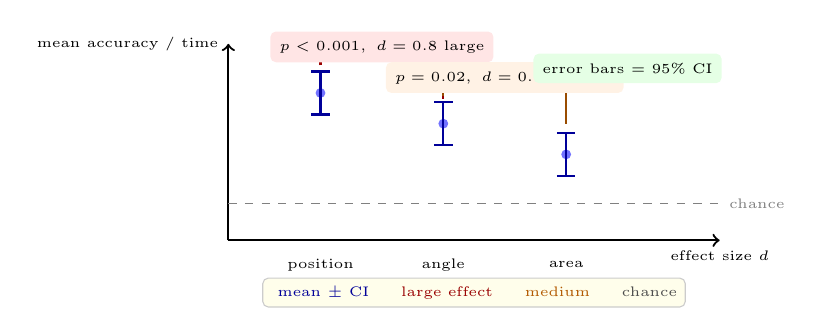
\begin{tikzpicture}[scale=0.78,every node/.style={font=\scriptsize}]
\draw[->,thick] (0,0) -- (8.0,0) node[below,font=\tiny] {effect size $d$};
\draw[->,thick] (0,0) -- (0,3.2) node[left,font=\tiny] {mean accuracy / time};
% conditions
\foreach \x/\y/\e/\lbl in {1.5/2.4/0.4/position, 3.5/1.9/0.45/angle, 5.5/1.4/0.5/area} {
  \fill[blue!55] (\x,\y) circle (0.08);
  \draw[thick,blue!60!black] (\x,\y-0.35) -- (\x,\y+0.35);
  \draw[thick,blue!60!black] (\x-0.15,\y-0.35) -- (\x+0.15,\y-0.35);
  \draw[thick,blue!60!black] (\x-0.15,\y+0.35) -- (\x+0.15,\y+0.35);
  \node[font=\tiny] at (\x,-0.4) {\lbl};
}
% significance brackets
\draw[thick,red!60!black] (1.5,2.85) -- (1.5,3.0) -- (3.5,3.0) -- (3.5,2.3);
\node[font=\tiny,fill=red!10,rounded corners=2pt] at (2.5,3.15) {$p<0.001,\ d=0.8$ large};
\draw[thick,orange!60!black] (3.5,2.35) -- (3.5,2.5) -- (5.5,2.5) -- (5.5,1.9);
\node[font=\tiny,fill=orange!10,rounded corners=2pt] at (4.5,2.65) {$p=0.02,\ d=0.4$ medium};
\node[font=\tiny,fill=green!10,rounded corners=2pt] at (6.5,2.8) {error bars = 95\% CI};
\draw[dashed,gray] (0,0.6) -- (8.0,0.6) node[right,font=\tiny] {chance};
\node[font=\tiny,draw=gray!40,fill=yellow!8,rounded corners=2pt,inner sep=3pt] at (4.0,-0.85) {\textcolor{blue!60!black}{$\blacksquare$ mean $\pm$ CI} \quad \textcolor{red!60!black}{$\blacksquare$ large effect} \quad \textcolor{orange!70!black}{$\blacksquare$ medium} \quad \textcolor{gray!60!black}{$\blacksquare$ chance}};
\end{tikzpicture}
\caption{Results as means with 95\% confidence intervals. Non-overlapping CIs signal a difference; report $p$-values and effect sizes ($d$), not just significance stars.}
\label{fig:results-ci}
\end{figure}

\begin{example}[Heer--Bostock replication sketch]\label{ex:heer}
Recruit 30 participants on a crowdsourcing platform. Within-subjects, each judges 20 ratio pairs per encoding (position, length, angle, area) in random order. DV: log absolute error $|\log(\text{judged}/\text{true})|$. Pilot shows $\sim$8\,s per trial. Analysis: mean log error per encoding with 95\% CI, repeated-measures ANOVA, post-hoc paired t-tests with Bonferroni, and Cohen's $d$.
\end{example}

\begin{lstlisting}[language=Python, caption={Analysing a two-condition study with CIs and t-test.}, label={lst:study-analyse}]
import numpy as np, scipy.stats as st, matplotlib.pyplot as plt

# synthetic: position more accurate than angle
np.random.seed(0)
pos = np.random.normal(0.12, 0.06, 30)   # log absolute error
ang = np.random.normal(0.22, 0.08, 30)
for name, arr in [("position",pos), ("angle",ang)]:
    m, se = arr.mean(), st.sem(arr)
    ci = se * st.t.ppf(0.975, len(arr)-1)
    print(f"{name}: mean={m:.3f} 95% CI [{m-ci:.3f},{m+ci:.3f}]")

t, p = st.ttest_rel(pos, ang)           # within-subjects
d = (pos-ang).mean() / (pos-ang).std(ddof=1)  # Cohen d (paired)
print(f"paired t={t:.2f} p={p:.4f} d={d:.2f}")

# plot means with CI
plt.figure(figsize=(4,2.5)); plt.errorbar([0,1],[pos.mean(),ang.mean()],
  yerr=[st.sem(pos)*st.t.ppf(0.975,29), st.sem(ang)*st.t.ppf(0.975,29)], fmt="o", capsize=6, color="steelblue")
plt.xticks([0,1],["position","angle"]); plt.ylabel("log absolute error"); plt.title("Means with 95% CI")
plt.tight_layout(); plt.savefig("ci.pdf")
\end{lstlisting}

\begin{lstlisting}[language=Python, caption={Power sketch and preference vs accuracy check.}, label={lst:power}]
import statsmodels.stats.power as smp

# how many participants for d=0.5, alpha=0.05, power=0.8 (paired)?
analysis = smp.TTestPower()
n = analysis.solve_power(effect_size=0.5, alpha=0.05, power=0.8, alternative="two-sided")
print(f"needed n ~ {n:.0f} per group (paired, so total N similar)")

# preference vs accuracy: people may prefer angle (familiar pie) but perform worse
# always report both; a scatterplot of preference rank vs error reveals the dissociation
\end{lstlisting}

% ============================================================
\section{Qualitative and Insight-Based Evaluation}
Not every question is a ratio judgment. For exploration, use \emph{insight diaries}, \emph{think-aloud}, and \emph{milestone} coding; for communication, test \emph{comprehension} and \emph{recall} after a delay. Qualitative data are coded by two raters with Cohen's $\kappa$ for agreement. Mixed methods---numbers plus quotes---often tell the full story.

% ============================================================
\section{Chapter Notes}
Pre-attentive and attention foundations from Treisman and Wolfe; change blindness from Simons and Levin; cognitive load from Sweller; Cleveland--McGill (1984) and Heer--Bostock (2010) set the evaluation standard for channels; Munzner (2014) framed evaluation across nested levels; Lam et al.\ (2012) catalogued seven evaluation scenarios. The final chapter turns evaluation into production.

% ============================================================
\section{Exercises}
\label{sec:ch07-exercises}
\begin{enumerate}[label=E7.\arabic*, leftmargin=*, itemsep=0.8em]
    \item \textbf{Pop-out design.} Design two searches on the same 30-item grid: one that pops out via colour alone and one that requires conjunction (colour+shape). Predict reaction time vs set size (4,16,30) for each and sketch the expected lines.
    \item \textbf{Study design.} Propose a within-subjects study comparing a rainbow vs a sequential palette for quantitative reading. State $H_0/H_1$, IV/DV, controls, number of trials, counterbalancing, and one threat (learning effect) with mitigation.
    \item \textbf{Analyse given data.} Two encodings produce log errors: A $[0.10,0.14,0.11,0.18,0.13]$ and B $[0.22,0.19,0.25,0.21,0.20]$. Compute means, 95\% CIs, paired t, and Cohen's $d$. Is the difference practically significant?
    \item \textbf{Power planning.} For a between-subjects comparison expecting $d=0.4$, $\alpha=0.05$, power $0.8$, estimate required $N$ per group. How does switching to within-subjects change $N$, and what new threat appears?
    \item \textbf{Insight diary.} Design an insight-based protocol for a visual analytics tool: task prompt, think-aloud instructions, insight coding rubric, and inter-rater reliability plan. When would this beat a timed accuracy study?
\end{enumerate}
% End of Chapter 7
